\documentclass[12pt]{article}
\usepackage{geometry}                % See geometry.pdf to learn the layout options. There are lots.
\geometry{letterpaper}                   % ... or a4paper or a5paper or ... 
\usepackage{graphicx}
\usepackage{amssymb}
\usepackage{amsthm}
\usepackage{epstopdf}
\usepackage[english]{babel}
%\usepackage[english, german]{babel}
\usepackage[utf8]{inputenc}
\usepackage[usenames,dvipsnames]{color}
\usepackage[table]{xcolor}
\usepackage{hyperref}
\usepackage{tikz}

\usepackage{wrapfig}
\usepackage{parskip}
\usepackage{subcaption}

\hypersetup{
    colorlinks=true,
    linkcolor=blue,
    filecolor=magenta,      
    urlcolor=cyan,
}

\DeclareGraphicsRule{.tif}{png}{.png}{`convert #1 `dirname #1`/`basename #1 .tif`.png}

\theoremstyle{definition}
\newtheorem{example}{Example}

\newenvironment{explanation}{%
   \setlength{\parindent}{0pt}
   \itshape
   \color{blue}
}{}

\newenvironment{text}{
   \setlength{\parindent}{0pt}
   \color{black}
}{}

\newcommand{\projectname}{Guideo}
\newcommand{\productname}{Vyzer}
\newcommand{\projectleader}{L. Engleder}
%\newcommand{\documentstatus}{In process}
\newcommand{\documentstatus}{Submitted}
%\newcommand{\documentstatus}{Released}
\newcommand{\version}{V. 1.2.31}

\begin{document}
\begin{titlepage}
\begin{flushright}

\includegraphics[scale=.5]{htlleondinglogo.png}\\
\end{flushright}

\vspace{10em}

\begin{center}
{\Huge System Specification} \\[3em]
{\LARGE \productname} \\[3em]
\end{center}

\begin{flushleft}
\begin{tabular}{|l|l|}
\hline
Project Name & \projectname \\ \hline
Product Name & \productname \\ \hline
Project Leader & \projectleader \\ \hline
Document state & \documentstatus \\ \hline
Version & \version \\ \hline
\end{tabular}
\end{flushleft}

\end{titlepage}
\section*{Revisions}
\begin{tabular}{|l|l|l|}
\hline
\cellcolor[gray]{0.5}\textcolor{white}{Date} & \cellcolor[gray]{0.5}\textcolor{white}{Author} & \cellcolor[gray]{0.5}\textcolor{white}{Change} \\ \hline
November 03, 2019&P. Bauer&First version \\ \hline
November 15, 2019&L. Engleder, L. Wirth, P. Quoc, A. Leeb & Initial Situation \\ \hline
November 18, 2019&L. Engleder, L. Wirth, P. Quoc, A. Leeb & Glossary and Use Cases \\ \hline
November 22, 2019&L. Engleder, L. Wirth, P. Quoc, A. Leeb & worked on Use Cases \\ \hline
November 25, 2019&L. Engleder, L. Wirth, P. Quoc, A. Leeb & overall improvements \\ \hline
December 6, 2019&L. Engleder, L. Wirth, P. Quoc, A. Leeb & worked on Use Cases \\ 
&& and System Architecture \\ \hline
December 13, 2019&L. Engleder, L. Wirth, P. Quoc, A. Leeb & worked on Use Cases \\ \hline
December 16, 2019&L. Engleder, L. Wirth, P. Quoc, A. Leeb & Overall improvements \\ \hline
December 17, 2019&L. Wirth & View description improvements \\ \hline
December 18, 2019&L. Engleder, L. Wirth, P .Quoc & worked on Use Cases and Model \\
&& of Application Domain \\ \hline
December 19, 2019&L. Engleder, L. Wirth, P .Quoc & worked on Use Cases, \\
&& overall improvements/fixes \\
&& and writing on the Acceptance \\
&& Criteria section \\ \hline
December 19, 2019&L. Engleder, L. Wirth, P .Quoch & proof reading \\ \hline

\end{tabular}
\pagebreak

\listoffigures
\pagebreak

\tableofcontents
\pagebreak

\section{Initial Situation and Goal}

\subsection{Initial Situation}

\begin{text}
There are still only a few ways for people to get information about their travelling destination.\newline

An established way is to read a physical or online travel guide. Depending on the creator they can be quite interesting and well constructed. Unfortunately, they are limited to the constraints of the written word. The recent rise of audio and video platforms has shown that many people consume educational content through these new mediums. Receiving the information in real-time also makes the experience of learning more enjoyable. It is also commonly known that there are different types of \href{https://www.tandfonline.com/doi/full/10.1080/0144341042000228834}{learning styles} and that many people learn more effectively through auditory stimulation over reading.\newline
 
Another option for many people is the possibility of hiring a tour guide or joining a bus tour, both promise to offer an educative personalized experience. 
First of all, there is a huge amount of people who are unable to take part in tours because of hearing impairment or slower walking speed.
For people who are travelling alone or with their families these tours can be quite expensive as the \href{https://www.guides-in-vienna.at/costs-terms//}{prices} are often fixed.
Since tours are conducted by humans, there are a few limitations by nature. A guide can only handle a certain amount of people per tour, while still having control of the big group. This is especially problematic when you consider that there are languages which are very sparsely if at all, supported. \href{https://linz-tours.at}{Linz Tours}, which provide tours in Linz, offer just one guide for Hungarian, Slovakian and Czech. They do not even support a single Asian language. Adding to that, it is possible that tour guides are fully booked, postponed or even cancelled.\newline
 
For many museums, the instalment of an audio guide system can be a big financial burden. Especially the purchase of custom hardware specialized companies seems out of place in our modern connected world. Moreover, a  high number of devices is needed if the museums want to offer audio guides to everyone. Popular events, like \href{https://www.tips.at/nachrichten/linz/kultur/459167-oberoesterreich-im-kunstfieber-schon-ueber-15-000-besucher-kamen-zu-den-grossen-meistern-in-die-tabakfabrik-linz}{the art exhibition in the Tabakfabrik Linz}, show how museums can be overwhelmed by the high amount of visitors and are therefore not able to provide every visitor with an audio guide.
Additionally, the headsets need to be cleaned properly at least after one use.
The headsets should not only look good, but they also need to be disinfected. Otherwise, \href{https://www.sciencedirect.com/science/article/abs/pii/S019607098580048X}{germs and viruses} stay on the earphones and will infect upcoming users. The most common method to get rid of a fraction of germs and viruses are simply by washing and cleaning the headsets with disinfecting alcohol, but this is not enough. To ensure the highest hygiene level a method called \href{https://www.ncbi.nlm.nih.gov/pmc/articles/PMC6379899/}{Ultraviolet Germicidal Irradiation} (UVGI) is a must. \href{https://pubs.asha.org/doi/abs/10.1044/jshr.1202.326}{UV irradiation} guarantees that nobody will get infected from using borrowed earphones. The problem is that most museums do not have these devices since they are quite expensive.
But without regular inspection and cleaning, these systems fail basic hygienic standards and also increase the chance of infecting visitors.
\newline

Although there are audio guides in use in museums there is still no way to enjoy them in a city in general. Our service would provide both locations with fitting guides.

Many guides are prearranged and have a fixed procedure. This grants the follower of the guide little to no flexibility. Even a quick trip to the toilet hinders the guiding group. If the guide is behind time, he will probably stress the people out and even skip some attractions and locations. \newline\newline

Since the inception of our project proposal, we made some decisions and changes, which aim to clarify and simplify things for the end-user. 

For example, we introduced the official status to distinguish between private verified users and official exhibition spaces. Official users enjoy more privileges and rights concerning their own facility and other guides. Moreover, we designed a more concrete verification and fact-checking system. Both of these examples are described in more detail in \hyperref[sec:verifyguides]{Verify and Fact Check Guides (Use Case 8)} and in
\hyperref[sec:disableguides]{ Disable other guides in their facility (Use Case 9)}.
\end{text}


\subsubsection{Application Domain}

\begin{text}
Our application mostly resides under the domain of culture, history and art. We need users that are interested in creating guides and informed about the subject they are going to create a guide about.  

One essential business process we have to integrate is the recruitment/partnership with museums, galleries and other exhibition spaces. These facilities help us reach a bigger audience while providing qualitative and informative content. 
We are in the process of contacting local museums and trying to build rapport with the people in charge of audio guides and technology in the respective facilities.

Generally, tourists are able to access and view guides through a variety of ways. Users can always view the guides in their current vicinity through the explorer view. 

Museums can for example display QR-Codes on the entrance of the museum to redirect the user directly to the guide. If the app is already open, it will also notify the user when entering a museum which offers a guide. 
\end{text}

\subsubsection{Glossary}

\begin{tabular}{|p{.2\linewidth}|p{.65\linewidth}|}
\hline
Track: & individual audio file giving information about one isolated sight or exhibit\\
\hline 
Audio Guide: & a collection of tracks aimed to tell a coherent story like a tour guide would  \\ 
\hline 
Verified Guide: & fact-checked guide made by a verified user, museum, gallery or other hosts\\ \hline
Tagging: & mapping each track with its respective monument or piece through Geo-location or QR-Codes  \\ 
\hline 
%Compilation/ & a combination of tracks from different audio guides and  \\ 
%Playlist & creators, like a music compilation\\
%\hline 
Verified User: &  privileged user with a record of factually correct content and expertise in a specific field\\ 
\hline 
Official User /  &  Museums, galleries, zoos and more that provide \\ 
Exhibition Spaces: & guides on the app. They have privileges regarding other guides in their building, prices and events.\\ 
\hline
Payment Method: & a way to process transactions for the purchase of guides \\
\hline
\end{tabular}

\pagebreak

\subsubsection{Model of the Application Domain}
\begin{figure}[hbt!]
    \label{fig:domain_cd}
    \centering
    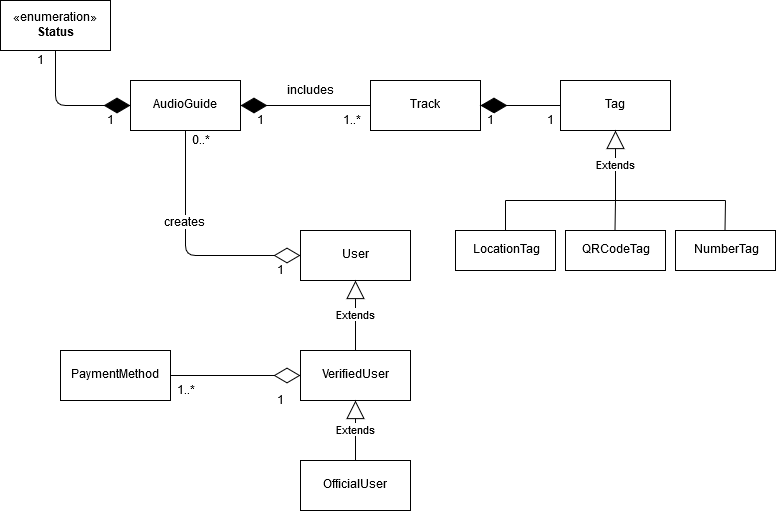
\includegraphics[width=0.85\textwidth]{ClassDiagram/ClassDiagramm_Domain.png}
    \caption{Application Domain Class Diagram}
\end{figure}

Status describes if the guide is a verified one.

\subsection{Goal}

\begin{text}
Our project aims to change the way we consume information while travelling. A modern approach to tourism is needed if we want to accommodate the sheer massive amount of people visiting sights, museums and galleries all over the globe. 

Our goal is to offer an affordable medium, which acts as a pocket local tour guide. This pocket tour guide can be individually specified so that anybody can have a perfect experience, just as they imagined. Due to the flexibility of the guides, a completely new experience emerges. It also enables people with physical disabilities like hearing impairment or people who struggle to keep up with the pace of the group. More specifically, people in wheelchairs and people with serious injuries. Those people should have the same breathtaking experience as a healthy user.

We want to provide as many languages as possible so that everybody can discover and explore the histories and cultures of the world. With the collective power of the community, we will be able to cover many more languages than any singular tourism business.

Another goal of this project is to free museums from buying, installing and maintaining expensive audio guide equipment. Especially, museums that organize big events suffer from lack of audio guide equipment and they tend to get damaged easily. Also, since many different visitors use one equipment within a day the equipment becomes unhygienic quickly. Our app will not suffer from such problems and should give museums a great possibility to switch from expensive hardware to a new affordable medium.
\end{text}

\pagebreak

\section{Functional Requirements}

\subsection{Overview: User Perspective}
\begin{figure}[hbt!]
    \centering
    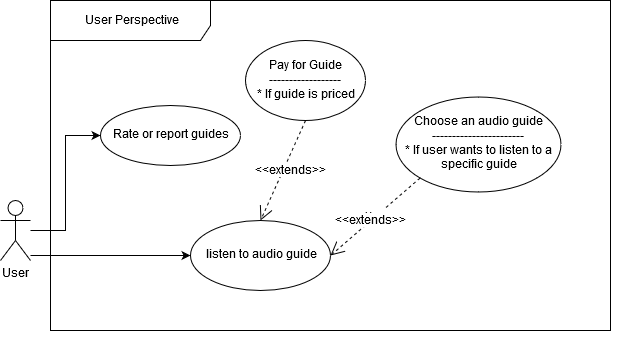
\includegraphics[width=0.9\linewidth]{UseCases/UserUseCase.png}
    \caption{User use cases}
    \label{fig:overview1}
\end{figure}

\subsection{Use Case 1: Rate or report guides}
    \subsubsection{General Description}
    
    \begin{tabular}{|p{.2\linewidth}|p{.65\linewidth}|}
        \hline 
        ID: & 001 \\ \hline
        Goal: & The user rates or reports a guide he listened to. \\ \hline
        Pre-condition: & The user has listened to a guide and decides to share their thoughts on their experience. \\ \hline
        Post condition: & The guide will have a new rating which will show if a user decides to look at it. \\ \hline
        Involved Users: & User: Listens to a guide and decides to rate or report it. \\ \hline
    \end{tabular}
    \pagebreak
    
    \subsubsection{UI to call the use case}
    \begin{figure}[hbt!]
        \centering
        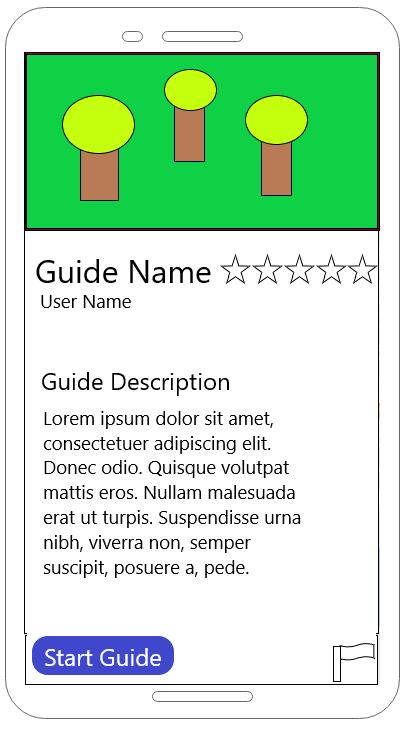
\includegraphics[width=0.35\linewidth]{UIs/GuideView.png}
        \caption{Guide Description View}
        \label{fig:guideview}
    \end{figure}
    
    \begin{text}
    The illustration above shows a normal guide view. The top of the illustration shows a forest (the guide creator can choose the picture he wants to be depicted here). Below that follows the guide name, next to it the rating and again below the guide name is the name of the guide creator. The stars are used to represent the rating. On the bottom right corner after the guide description (which is written by the guide creator) is a flag, which is used to report the guide (for distribution of fake facts or other reasons).
    
    If the user clicks on the listen button he will be sent to the \hyperref[fig:usecase2]{listening view} and will listen to the first track of that guide. 
    \end{text}
    
    \subsubsection{The Standard Use}
    \begin{text}
    Rate: The user clicks on one of the stars to rate the guide 1-5 stars.
    
    \begin{figure}[hbt!]
        \centering
        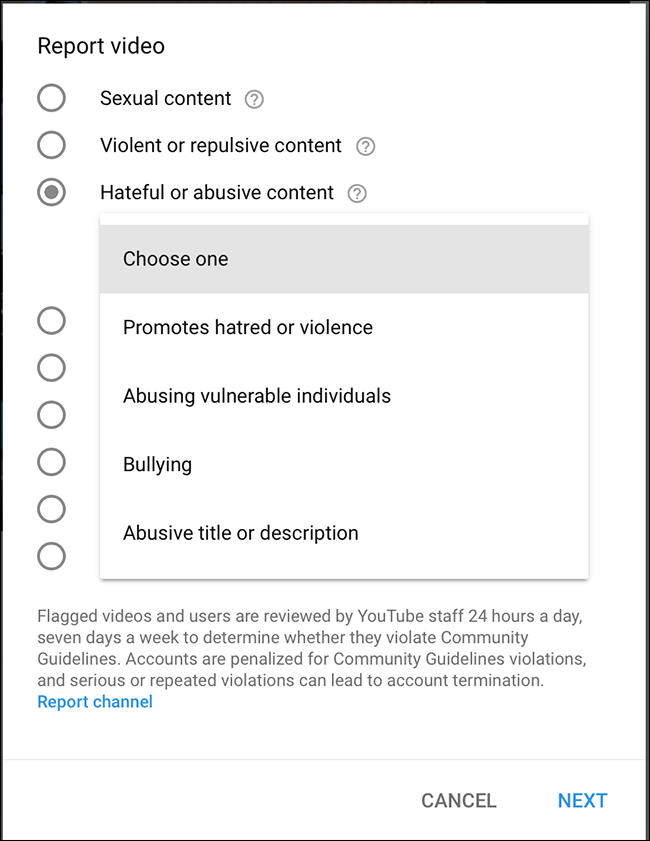
\includegraphics[width=0.5\linewidth]{UIs/reporting_ui.png}
        \caption{Reporting a Guide (source: Youtube)}
        \label{fig:reporting_ui}
    \end{figure}
    Report: The user clicks on the report flag to open a report-popup, state the reason for the report and send it to the server.
    
    In the standard use, the guide will receive a new rating or will be reported for admins to review.
    \end{text}
    
    \subsubsection{The Non-Standard Use}
    \begin{text}

    No Signal: \hyperref[sec:gnsu]{See section General Non-Standard Uses }
    
    Guide is not available : \hyperref[sec:gnsu]{See section General Non-Standard Uses }
    \end{text}
    
\pagebreak

\subsection{Use Case 2: Listen to audio guides}
    \subsubsection{General Description}
    
    \begin{tabular}{|p{.2\linewidth}|p{.65\linewidth}|}
        \hline 
        ID: & 002 \\ \hline
        Goal: & The user uses the app to listen to the tracks of an audio guide \\ \hline
        Pre-condition: & The user chose an audio guide, scanned a QR-Code or activated auto-play \\ \hline
        Post condition: & After the user has listened to the tracks of the guide, he is able to rate or report the guide \\ \hline
        Involved Users: & User: Listens to the tracks of an audio guide \\ \hline
    \end{tabular}
    
    \subsubsection{UI to call the use case}
    \begin{figure}[hbt!]
        \label{fig:usecase2}
        \centering
        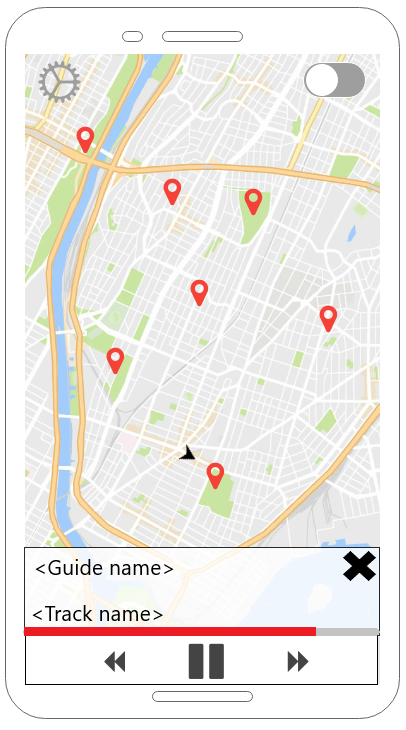
\includegraphics[width=0.35\linewidth]{UIs/ListeningView.PNG}
        \caption{Listen to a guide View}
    \end{figure}
    \begin{text}
    The illustration above shows the view that appears while the user is listening to a guide if the app is open.
    
    Clicking on the wheel at the top left corner brings the user to the options view. At the top right corner, the user can toggle on or out the auto-play option.
    
    The user is displayed as a black arrow on the map. Depending on the situation the red pins have a different meaning. If the user is currently listening to a guide, the red pins are the positions of the guide's tracks. If the user is not listening, the red pins are the positions of the first track of the audio guides that are displayed.
    
    Some information about the current guide and the current playing track are displayed at the bottom of the view. A progress bar shows how much of the tracks time has passed. The user has also the possibility to cancel the current guide. 
    
    If the user clicks on a pin some information about the track/guide (depending on the situation) will be displayed.
    
    If the user swipes to the left, he will be sent to the explorer view described in \hyperref[sec:gnsu]{Use Case 3: Choose an audio guide}
    \end{text}
    
    \subsubsection{The Standard Use}
    \begin{text}
    The user listens to the complete guide without having to touch his phone. The tracks are played automatically when the user walks by a sight, where the track is placed. There are no disturbances or breaks needed and the connection to the internet is perfectly stable.
    
    If the app is active, the user has the possibilities described in 'UI to call the use case'.
    
    Look for
    \hyperref[fig:listen_act_dg]{this}
    state diagram for the detailed process.
    \end{text}
    
    \begin{figure}
        \vspace*{-3cm}
        \centering
        \label{fig:listen_act_dg}
        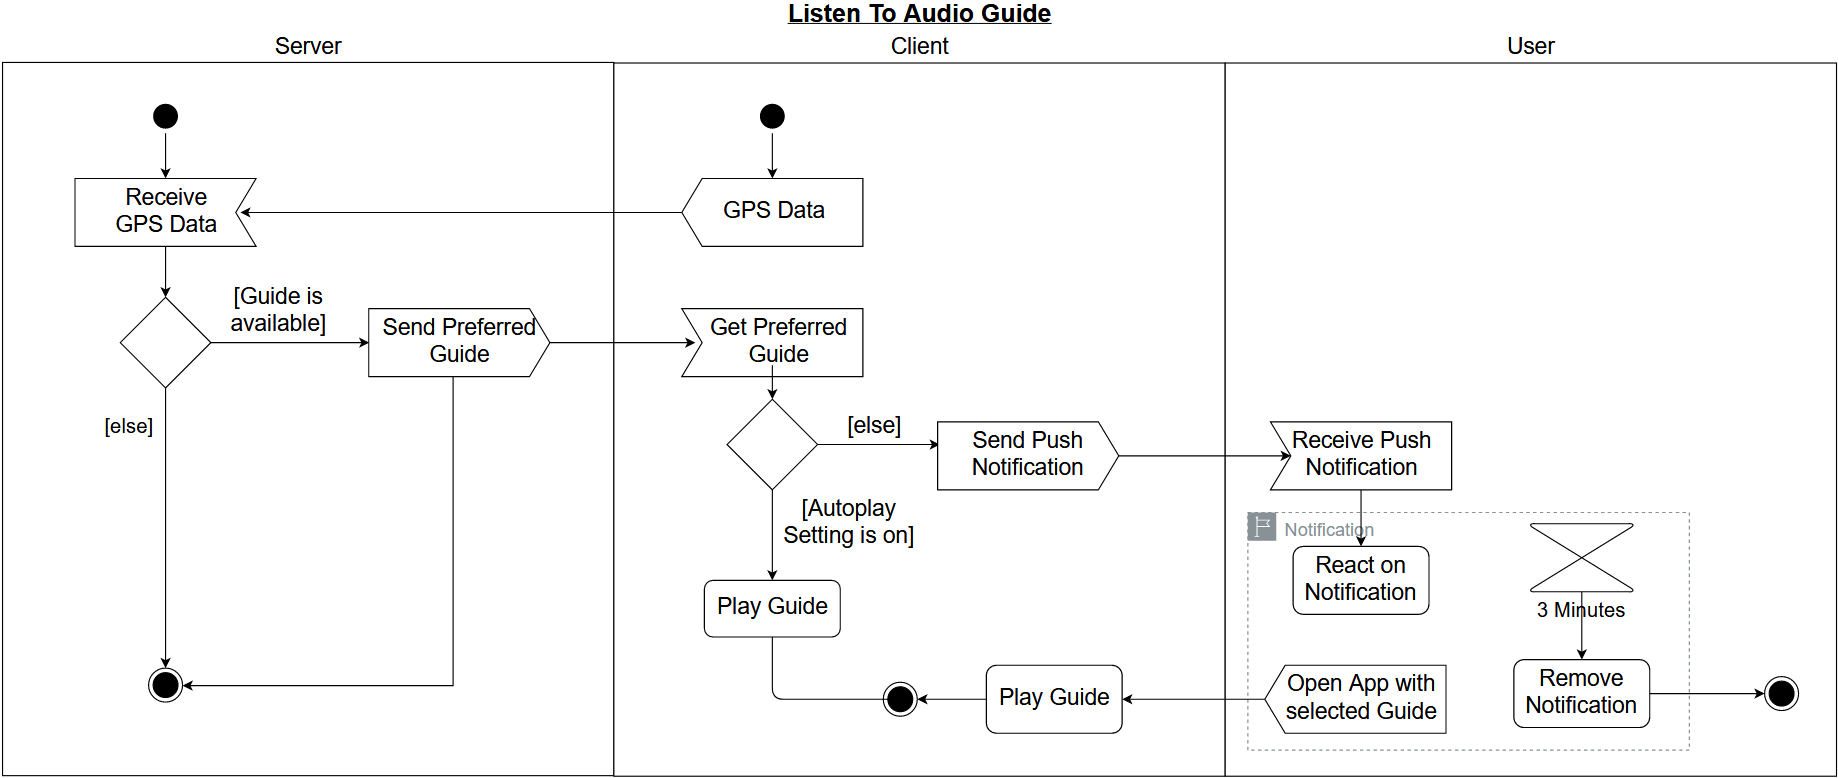
\includegraphics[width=1.1\textheight,
       angle=90]{ActivityDiagram/GuideListeningAD.png}
        \caption{Activity Diagram Listen to Guide}
    \end{figure}
    
    \subsubsection{The Non-Standard Use}
    \begin{text}
    
    No Signal: \hyperref[sec:gnsu]{See section General Non-Standard Uses }
    
    Guide is not available : \hyperref[sec:gnsu]{See section General Non-Standard Uses }
    \end{text}
\pagebreak

\subsection{Use Case 3: Choose an audio guide}
\label{chooseguide}
    \subsubsection{General Description}
    
    \begin{tabular}{|p{.2\linewidth}|p{.65\linewidth}|}
        \hline 
        ID: & 003 \\ \hline
        Goal: & to select a specific audio guide out of preference in order to listen to it. Otherwise the user has to activate autoplay \\ \hline
        Pre-condition: & being in a location, where audio guides are located \\ \hline
        Post condition: & An audio guide is selected and ready to listen for \\ \hline
        Involved Users: & User: Wants to choose an audio guide to listen to \\ \hline
    \end{tabular}
    
    \subsubsection{UI to call the use case}
    \begin{text}
    There is not really a UI to call the use case. If the user finished the login process, he will automatically be sent to the \hyperref[fig:map_view]{map view}. From there the user can navigate to the Explorer View.  
    \end{text}
    
    \subsubsection{The Standard Use}
    \begin{figure}[hbt!]
        \begin{subfigure}{0.5\textwidth}
            \centering
            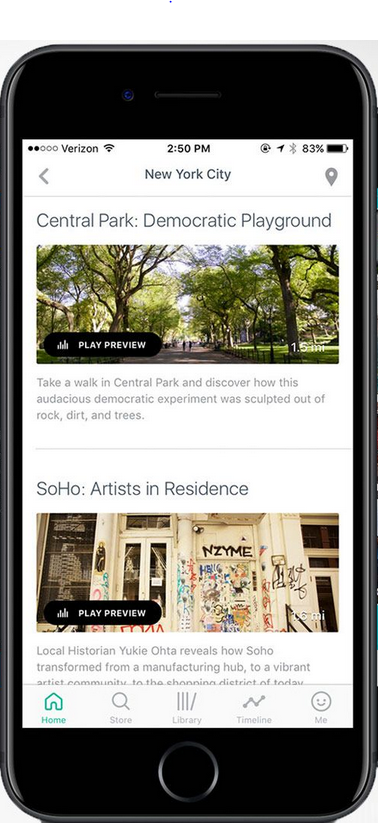
\includegraphics[width=0.5\linewidth]{UIs/ExplorerView1.PNG}
            \caption{Explorer View 1}
            \label{fig:ex_view_1}
        \end{subfigure}
        \begin{subfigure}{0.5\textwidth}
            \centering
            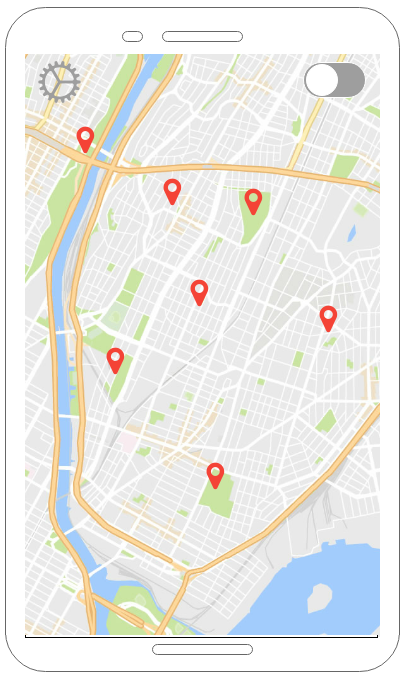
\includegraphics[width=0.6\linewidth]{UIs/MapView.png}
            \caption{Map View}
            \label{fig:map_view}
        \end{subfigure}
        \caption{Ways to choose an audio guide}
    \end{figure}
    
    \begin{text}
    The explorer view displays all guides that feature a track in a 1km radius. This includes guides by independent creators and all verified and official guides. 
    
    Basically, the view consists of a simple list with sorting and filtering options. By pressing on a guide one can see a more detailed description with the option to play the guide directly. The user can also choose to display guides in a bigger radius or in a specific city.
    \end{text}
    
    \subsubsection{The Non-Standard Use}
     \begin{text}
    There are no guides in this area available: the app shows, instead of the guides, a message telling the user that there, unfortunately, are no guides in his/her vicinity
    
    No Signal: \hyperref[sec:gnsu]{See section General Non-Standard Uses }
    
    Guide is not available : \hyperref[sec:gnsu]{See section General Non-Standard Uses }
    \end{text}
    
\subsection{Use Case 4: Pay for Guide}
    \subsubsection{General Description}
    
    \begin{tabular}{|p{.2\linewidth}|p{.65\linewidth}|}
        \hline 
        ID: & 004 \\ \hline
        Goal: & Pay for guide in order to be able to listen to its tracks \\ \hline
        Pre-condition: & Creator of the guide  set a price and specified a payment method \\ \hline
        Post condition: & User is able to listen to the guide's tracks \\ \hline
        Involved Users: & User: Pays for a guide he wants to listen to \\ \hline
    \end{tabular}
    
    \subsubsection{UI to call the use case}
    \begin{text}
    The UI to call this Use Case has many similarities with Guide Description View. The User will be informed that the guide he chose is to be purchased with information on the guide view itself. Additionally, when the user decides to purchase the guide there will be a pop-up where he has to confirm that he wants to purchase it.
    \end{text}
    
    \subsubsection{The Standard Use}
    \begin{text}
    The user chooses a provider (e.g. PayPal) for the transfer. The payment method has to be compatible with the payment methods, which were chosen by the creator of the guide. If the user has not already either specified his account/bank data by defining them at the account registration or used other methods like Google Play/Billing, he will be prompted to enter his payment details
    
    After that, the money will be transferred to the creators' bank account.   
    \end{text}
    
    \subsubsection{The Non-Standard Use}
    \begin{text}
    Billing details are wrong: The money cannot be transferred due to incorrect bank/account information. This could be true for either the user or the creator of the guide.
    
    Transaction failed: Because of external causes, the transaction was not successfully finished. Reasons may include a blocked bank account, not enough money, etc.
    \end{text}
    
\pagebreak

\subsection{Overview: Management Perspective }

\begin{figure}[hbt!]
    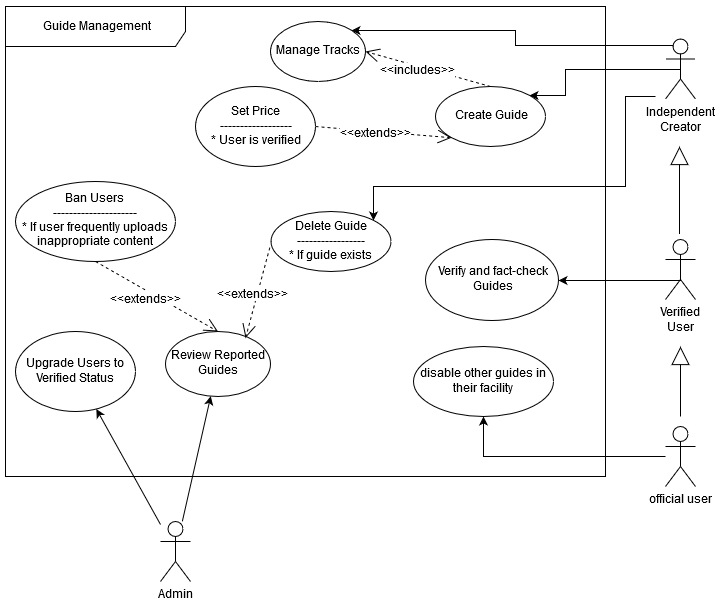
\includegraphics[width=1\linewidth]{UseCases/ManagementUseCases.png}
    \caption{Guide Management use cases}
    \label{fig:overview2}
\end{figure}
\begin{text}
A verified user can do everything what an independent creator can. Therefore a official user can do everything what an verified user can and more.

But with being a verified user, comes great responsibility. Keeping a written transcript and constantly reviewing and fact-checking guides are the two features that aim to improve the quality of the content. Verified users have to adhere to these rules to create guides with verified status.
\end{text}

\subsection{Use Case 5: Create Guide}
    \subsubsection{General Description}
    
    \begin{tabular}{|p{.2\linewidth}|p{.65\linewidth}|}
    \hline 
    ID: & 005 \\ \hline
    Goal: & A guide will be added to the system \\ \hline
    Precondition: & The user wants to create a guide \\ \hline
    Postcondition: & The guide is available for other users \\ \hline
    Involved Users: & Guide creator: User who wants to create a guide\\ \hline
    \end{tabular}
    
    \subsubsection{UI to call the use case}
    \begin{figure}[hbt!]
        \centering
        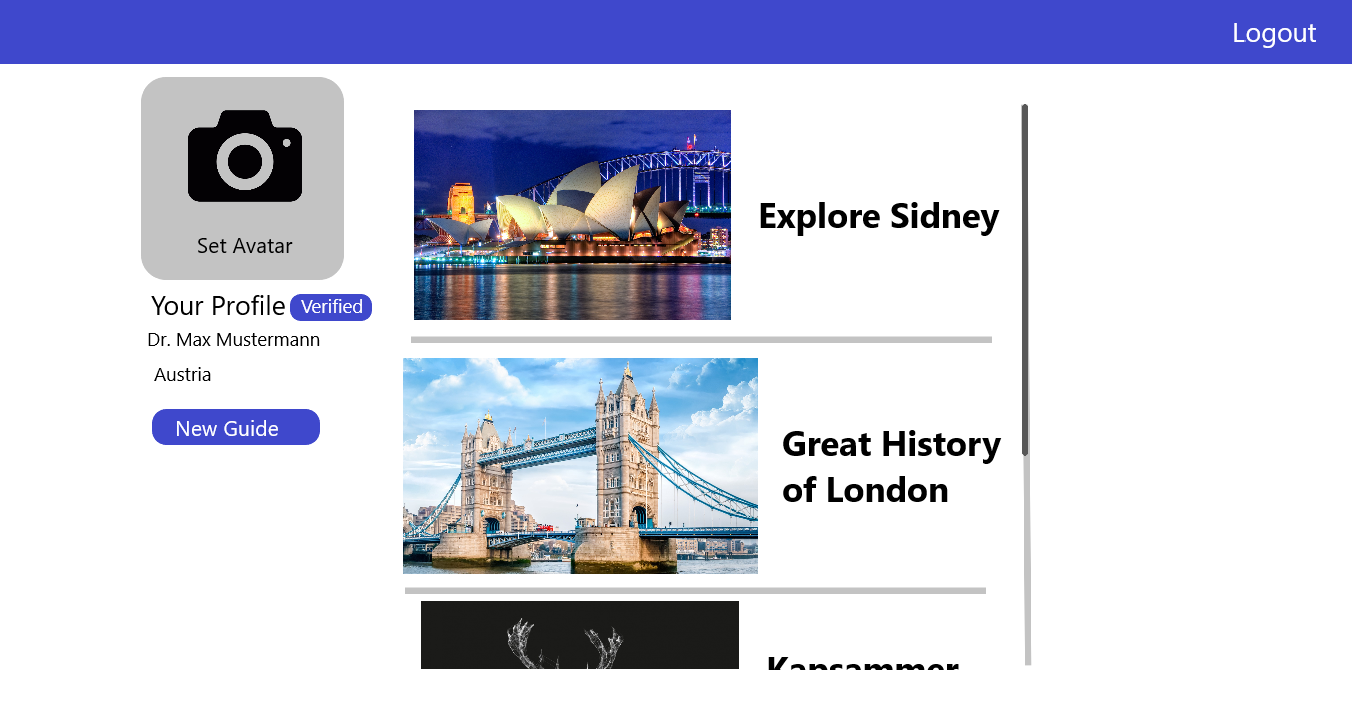
\includegraphics[width=1\linewidth]{UIs/ProfileWeb.png}
        \caption{Profile View}
        \label{fig:profile_view}
    \end{figure}
    \begin{text}
    This picture above shows the structure of the explorer view on the webpage. It shows some general information regarding the person behind the account on the left. Moreover, his status is also displayed. The user can scroll through the guides he already created in the middle of the website. By clicking on one of these guides he will be sent to the guide description view.
    
    Furthermore, he can click on the new guide button to create a new guide. After that action he will be sent to the \hyperref[fig:create_guide]{guide creation view}. All users are able to check out the profile page of other users (of course without the new guide button).
    \end{text}
    \subsubsection{The Standard Use}
    \begin{figure}[hbt!]
        \label{fig:create_guide}
        \centering
        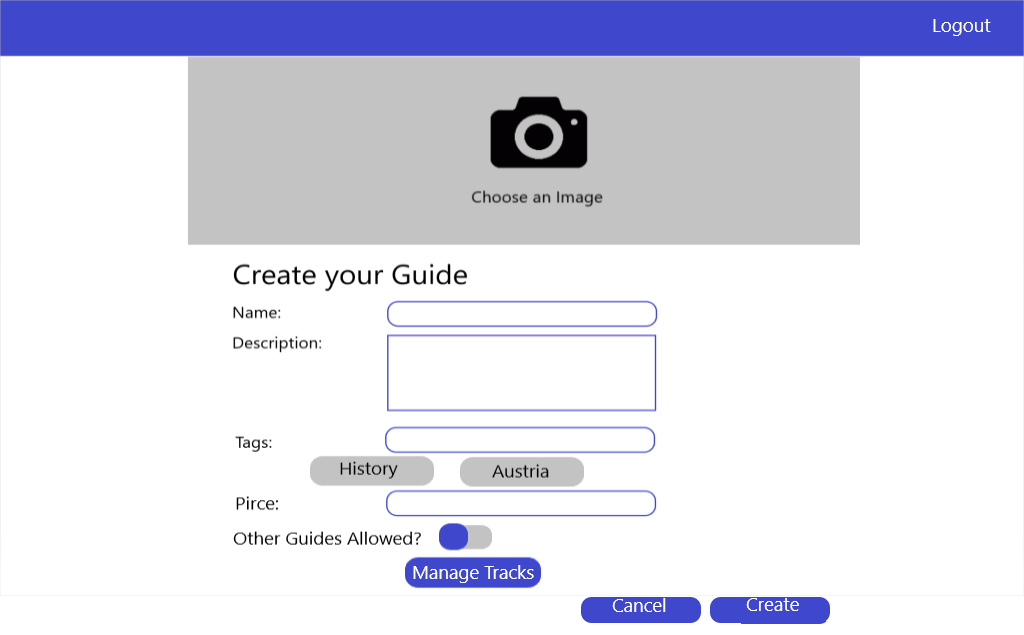
\includegraphics[width=1\linewidth]{UIs/CreateGuideWeb.PNG}
        \caption{Create Guide View}
    \end{figure}
    \begin{text}
    The create guide feature will only be supported on the website for desktop devices.
    The user gets taken through different stages in the creation process. 
    First, he will be prompted to define a title and a simple description. Then he gets taken to  
    "Manage Tracks" where he has to upload tracks and map them to the right location.
    Furthermore, specific roles have additional customized options, for example, official users can disable other guides in their facility.
    \end{text}
    \subsubsection{The Non-Standard Use}
    \begin{text}
    If the creator does not specify a title or a description an error message will get shown, prompting him or her to complete the fields.
    \begin{figure}[hbt!]
        \centering
        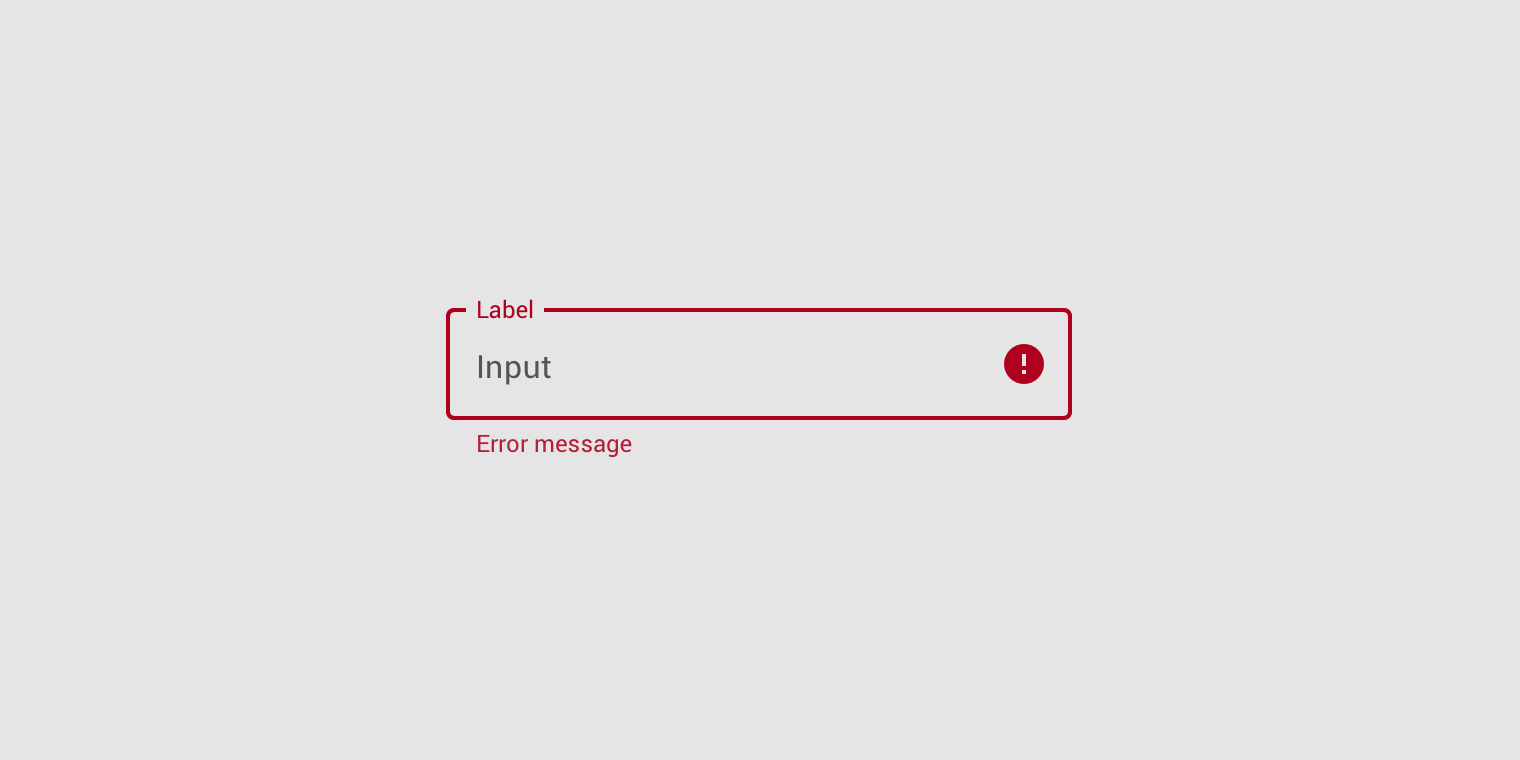
\includegraphics[width=1\linewidth]{UIs/text-field-error.png}
        \caption{Text field error}
        \label{fig:text-field-error}
    \end{figure}
    
    For all file and location related errors: \hyperref[sec:managetracks_nsu]{See section to non-standard uses in Manage Tracks }
    
    For No-Signal: \hyperref[sec:gnsu]{See section General Non-Standard Uses }.
    Moreover, the process will be paused and the user will be able to continue 
    \end{text}

\subsection{Use Case 6: Manage Tracks}
    \subsubsection{General Description}
    \begin{tabular}{|p{.2\linewidth}|p{.65\linewidth}|}
    \hline 
    ID: & 006 \\ \hline
    Goal: & Change the order of the tracks, add and remove any tracks \\ \hline
    Precondition: & The user is creating a guide or he wants to modify an already existing guide \\ \hline
    Postcondition: & Other users can access the new or updated guide  \\ \hline
    Involved Users: & Guide manager: A User who has created a/some guide/s previously and now wants to manage them.\\ \hline
    \end{tabular}
    
    \subsubsection{UI to call the use case}
    \begin{text}
    If the user clicks on the Manage Tracks Button from the \hyperref[fig:create_guide]{Create Guide View} or if he clicks on the Manage Tracks Button in the guide View, he will be sent to the Manage Tracks View.
    \end{text}
    \newline
    \newline
    
    \subsubsection{The Standard Use}
    \begin{text}
    After deciding on the title and general settings of the guide the creator will have to upload his tracks to the platform. These tracks have to be mapped to their specific location or tagging value. The uploading faces no delays. These tracks can also be edited/reset after creation. Also, it is possible to add/remove tracks afterwards.  
    \end{text}
    
    \subsubsection{The Non-Standard Use}
    \label{sec:managetracks_nsu}
    \begin{text}
    If a file does not have the correct file format, is too big or is somehow corrupted, the track will appear red and display a small message stating the error concerning the file.
    
    If the creator does not specify a location or tag for a specific track he will be notified that each track has to have a corresponding location or tag.
    \end{text}

\subsection{Use Case 7: Set Price}
    \subsubsection{General Description}

    
    \begin{tabular}{|p{.2\linewidth}|p{.65\linewidth}|}
    \hline 
    ID: & 007 \\ \hline
    Goal: & To configure the price any other payment settings \\ \hline
    Precondition: & The user is an official user \\ \hline
    Postcondition: &  A fixed price is set and the guide can be bought. \\ \hline
    Involved Users: & Verified creator: A User who is verified, has created a/some guide/s previously and now wants to set a price for them. \\ \hline
    \end{tabular}
    
    \subsubsection{UI to call the use case}
    \begin{text}
    This Use Case can be reached by the same \hyperref[fig:create_guide]{Create Guide View} as in Use Case 5. There is just another option for setting a price.
    \end{text}
    
    \subsubsection{The Standard Use}
    \begin{text}
    In this step of the guide creation the official or verified user is prompted to configure the available payment transfer options. For each payment option he will have to specify his account/bank information. He can also link his Google Pay account to simplify the matter. 
    
    More importantly, he has to decide on a fixed priced for his guide. 
    The user will be informed about the average prices of guides in his area and the specifics of our provision-based business model.
    \end{text}
    
    \subsubsection{The Non-Standard Use}
    \begin{text}
    
    No Signal: \hyperref[sec:gnsu]{See section General Non-Standard Uses } 
    The creation of the guide will be continued after the connection issues have been resolved.
    
    Incorrect Bank/Account details: The user will be prompted to either remove the payment option or to correct his faulty info. A small error message appears on the screen.
    
    No Payment Option: If the user wants to sell a guide, he has to specify a payment option. Before continuing the guide creation process an error message will appear, prompting the creator to enable some way of paying. 
    
    \end{text}

\subsection{Use Case 8: Verify and fact-check guides}
\label{sec:verifyguides}
    \subsubsection{General Description}
    
    
    \begin{tabular}{|p{.2\linewidth}|p{.65\linewidth}|}
    \hline 
    ID: & 008 \\ \hline
    Goal: & The goal of the use case \\ \hline
    Precondition: & Under which condition is the user case triggered? \\ \hline
    Postcondition: & What conditions are true after the use case was successfully executed? \\ \hline
    Involved Users: & Inspector: A verified user who reviews and then verifies or fact-checks guides. \newline
    Verified Creator: He/She created a presumably flawed guide.\\ \hline
    \end{tabular}
    
    \subsubsection{UI to call the use case}
    
    \subsubsection{The Standard Use}
    \begin{text}
    To insure the quality and correctness of verified guides, we devised a system of consecutive fact-checks and corrections. Basically, when a verified user creates a guide, it has verified status. Other verified users can request changes if needed. Through the change and the addition of sources these errors can be corrected. 
    
    Moreover, this process can always be ended through the deletion of the guide.
    \end{text}
    
    \begin{figure}[hbt!]
    \centering
    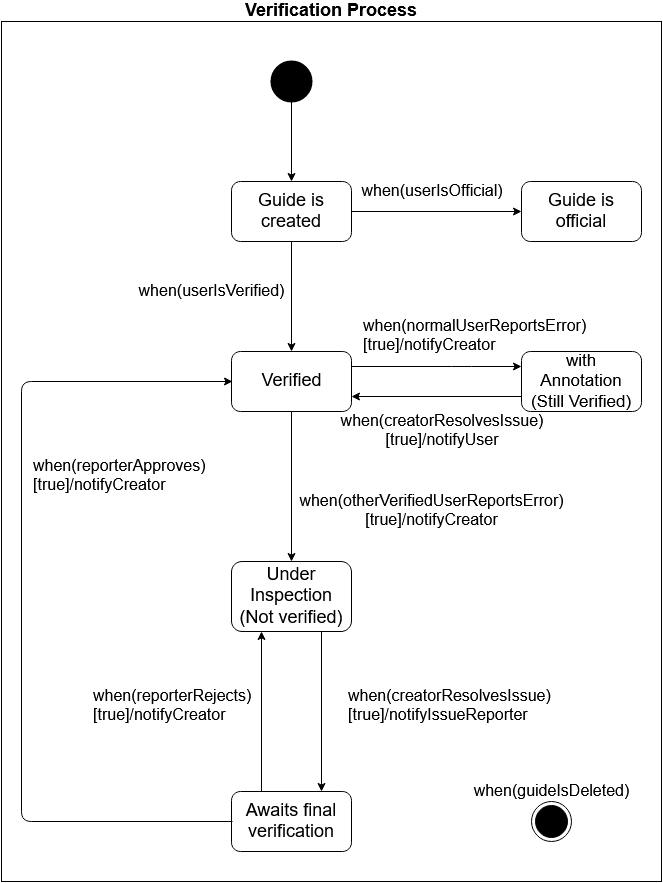
\includegraphics[width=0.8\linewidth]{StateDiagram/GuideVerificationSD.png}
    \caption{Verify Guides}
    \label{fig:verifyguides_sd_dg}
    \end{figure}
    
    \pagebreak

    \subsubsection{The Non-Standard Use}
\begin{text}
Although the system is designed to ensure quality through the involvement of multiple people, there can still be users who will take advantage of the system.

Wrong Correction: Users could request a correction for things, that do not need correction to downgrade the status of the guide.

Verification Inactivity: Verified users do not contribute to the ä--system.

Multiple Accounts/Bots: Users could create more accounts to harass creators with constant change requests
\end{text}

\subsection{Use Case 9: Disable other guides in the facility}
\label{sec:disableguides}
    \subsubsection{General Description}
    
    \begin{tabular}{|p{.2\linewidth}|p{.65\linewidth}|}
    \hline 
    ID: & 009 \\ \hline
    Goal: & The goal of the use case \\ \hline
    Precondition: & The user has official status and there are other independent guides in their facility \\ \hline
    Postcondition: & Inappropriate or unwanted guides are no longer shown, when a user enters the exhibition space \\ \hline
    Involved Users: & Official Creator: An Official Creator can disable other guides in their own facility. \newline
    User: He/She cannot create any guide within that area.\\ \hline
    \end{tabular}
    
    \subsubsection{UI to call the use case}

    
    \subsubsection{The Standard Use}
    \begin{text}
    Generally, there are no limits for the locations of guides. But museums and galleries will have the possibility of deactivating independent guides in their facility. Some of them may want to only support their own official guide. Others may want to prevent the publication of any inappropriate or political charged content at sensitive memorial sites.
    
    The people responsible will be able to see a list of all the guides that contain locations inside or in near proximity of the respective museum. Through a simple click, the specific tracks will be disabled inside of the facility. The creator of the guide will be notified and has the option to remove or revise his tracks.
    
    \end{text}
    
    \subsubsection{The Non-Standard Use}
    
    No Signal: \hyperref[sec:gnsu]{See section General Non-Standard Uses } 

\subsection{Use Case 10: Upgrade Users to Verified/Official Status}
    \subsubsection{General Description}
    \begin{tabular}{|p{.2\linewidth}|p{.65\linewidth}|}
    \hline 
    ID: & 010 \\ \hline
    Goal: & Upgrade normal users to verified status \\ \hline
    Precondition: & If an admin decides that a normal user has published enough professional content to deserve verified status \\ \hline
    Postcondition: & The user has verified status and has to obey the presented guidelines\\ \hline
    Involved Users: & Admin: Will grant an user the verified status.
    User: He/She applies for the verified status. \\ \hline
    \end{tabular}
    
    \subsubsection{UI to call the use case}
    
    \subsubsection{The Standard Use}
    \begin{text}
    Independent users can apply through email to be considered for verified status. This includes sending in references, proof of academic career and other general information. After reviewing the already created guides and the additional documents which were sent in, the admin can upgrade the user through an interface. 
   
   He simply finds the user by his email or username and upgrades his status. With the status change the user will receive an email, confirming his status change. In the email, the user will be redirected to a page that explains the rules and guidelines when creating a verified guide.
   
   
   Nearly the same is applicable to museums and other exhibition spaces. Although, the application of official users does not include a real review of their accomplishments. It is more of a proof of existence.
    \end{text}
    
    \subsubsection{The Non-Standard Use}
    \begin{text}
    
    Username not found: The user will be notified that the specified email is incorrect.
    
    Application denied: The user will be informed of the rejection
    \end{text}

\subsection{Use Case 11: Review Reported Guides}
    \subsubsection{General Description}
    
    \begin{tabular}{|p{.2\linewidth}|p{.65\linewidth}|}
    \hline 
    ID: & 011 \\ \hline
    Goal: & Displaying the content of the guide and showing why and by whom it was reported\\ \hline
    Precondition: &  The specific guide was reported\\ \hline
    Postcondition: & Deleting the respective guides\\ \hline
    Involved Users: & Admin/Supervisor: A user who has permission to review and delete/disable a guide. \newline
    Creator: The creator of the reported guide. \\ \hline
    \end{tabular}
    
    \subsubsection{UI to call the use case}
    \begin{text}
    \end{text}
    
    \subsubsection{The Standard Use}
    \begin{text}
    The admins have a list of reported guides. They review the reported guides on the grounds of the report. If a report is justified the admin can remove the guide. This can in a wider sense lead to the ban of a User, whose guides have been reported and removed repeatedly.
    \end{text}
    
    \subsubsection{The Non-Standard Use}
    \begin{text}
    Guide is not available : \hyperref[sec:gnsu]{See section General Non-Standard Uses }
    \end{text}

\subsection{Use Case 12: Disable or Delete Guide}
    \subsubsection{General Description}
    \begin{tabular}{|p{.2\linewidth}|p{.65\linewidth}|}
    \hline 
    ID: & 012 \\ \hline
    Goal: & The is not available for users  \\ \hline
    Precondition: & The guide was thoroughly reviewed\\ \hline
    Postcondition: & The guide cannot be accessed by users and is not visible in the app. \\ \hline
    Involved Users: & Admin: Wants to disable a guide \newline
Creator: Created the guide or wants to delete his guide \\ \hline
    \end{tabular}
    \newline
    
    \newpage
    \subsubsection{UI to call the use case}
    \begin{text}
    This Use Case has a similar UI as \hyperref[fig:create_guide]{Create Guide View} in Use Case 5. Just with added buttons to disable/delete the created guide.
    \end{text}
    
    \subsubsection{The Standard Use}
    
    \begin{text}
    In order to delete or disable a guide, the user has to select the guide out of a list view. The admin can delete guides by either searching for the user or deleting the guide with its guide id.
    \end{text}
    
    \subsubsection{The Non-Standard Use}
\begin{text}
    Guide is not available : \hyperref[sec:gnsu]{See section General Non-Standard Uses }, maybe it was already deleted
\end{text}

\subsection{Use Case 13: Ban Users}
    \subsubsection{General Description}
    \begin{tabular}{|p{.2\linewidth}|p{.65\linewidth}|}
    \hline 
    ID: & 013 \\ \hline
    Goal: & Ban the user from the platform  \\ \hline
    Precondition: & Due to many violations against the policy, a supervisor will ban the user\\ \hline
    Postcondition: & The user has been successfully banned from the system.\\ \hline
    Involved Users: & User: The user, who published multiple guides and violated one or many guidelines in the process.
    Supervisor/Admin: Person who is responsible for banning the user. \\ \hline
    \end{tabular}
    
    \subsubsection{The Standard Use}
    \begin{text}
The supervisor/admin can access a list with all the users that already have three guides that were condemned as inappropriate. He/She will review every creator to confirm the violations and will, therefore, ban the user from creating any more content.
    \end{text}
    
    \subsubsection{The Non-Standard Use}
    \begin{text}
    User not available: The user account has already been deleted.
    \end{text}
\pagebreak

\section{General Non-Standard Uses}
\label{sec:gnsu}
\subsection{Non-Standard Use 1: No Signal}
    \begin{figure}[hbt!]
        \centering
        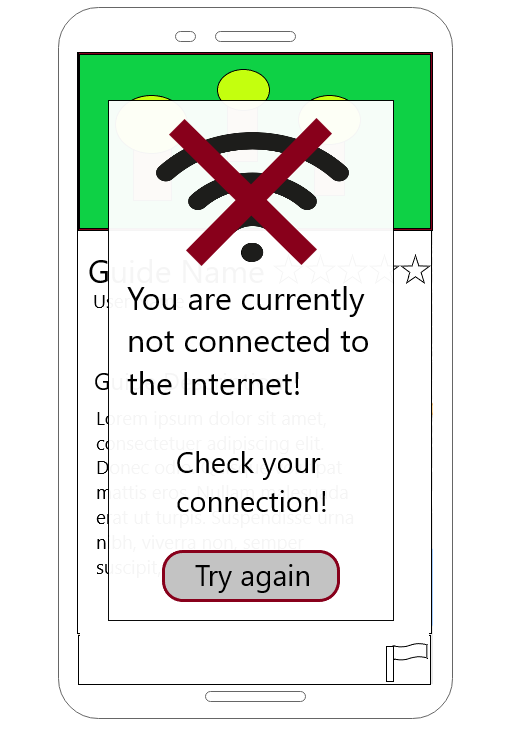
\includegraphics[width=0.35\linewidth]{UIs/NoWifiSignal.png}
        \caption{No Signal View}
        \label{fig:usecase1}
    \end{figure}
    \begin{text}
    This UI shows up, when you have no internet access. If the user checks his internet connection he can use the button at the bottom to try to establish a connection to our server again. If the try succeeds the pop-up will disappear, otherwise it will stay up.
    \end{text}
\subsection{Non-Standard Use 2: Guide is not available}
    \begin{text}
    The guide is not available(w/o UI):
    If the guide, for any reason, is not available anymore, the user will not be able to interact with it. The user is, after a quick error message pop-up, brought back to the primary UI.
    \end{text}
    
\pagebreak

\section{Non-Functional Requirements}

\subsection{NFR 1: User data}
    \begin{tabular}{|p{.2\linewidth}|p{.65\linewidth}|}
    \hline 
    ID: & NFR-001 \\ \hline
    Name: & User data Security \\ \hline
    Type    : & SEC \\ \hline
    Description: & We have to consider about security, for example, for the payment processes of our app. Secure bank account data should not be available to third party users. Also other user data like account password should not be readable for unauthorised people. \\ \hline
\end{tabular}

\subsection{NFR 2: Easy Guide Access}
    \begin{tabular}{|p{.2\linewidth}|p{.65\linewidth}|}
    \hline 
    ID: & NFR-002 \\ \hline
    Name: & Easy Guide Access \\ \hline
    Type    : & USE \\ \hline
    Description: & Guides on the guide view nearby the user should be easy to access for the user, since the user does not want to waste time on the UI. Most of guide configuration options should be found on the same page, since creators want change the options quickly.  \\ \hline
\end{tabular}

\subsection{NFR 3: Playing Tracks}
\begin{tabular}{|p{.2\linewidth}|p{.65\linewidth}|}
\hline 
ID: & NFR-003 \\ \hline
Name: & Playing Tracks \\ \hline
Type    : & EFFIC \\ \hline
Description: & 
Tracks should be played fluently, so there is no long delay due to loading times between the current track and the next track. In case of an unstable connection, the track should still be played reasonably smooth, without any consistent stuttering or annoying pauses. \\ \hline
\end{tabular}

\subsection{NFR 4: Maintainability}
\begin{tabular}{|p{.2\linewidth}|p{.65\linewidth}|}
\hline 
ID: & NFR-004 \\ \hline
Name: & Maintainability \\ \hline
Type    : & MAINT \\ \hline
Description: & Since this idea is a big project with many features, we have create a easy extendable software architecture and we have to document its implementation. This should make further implementation and work on our software easier. \\ \hline
\end{tabular}

\pagebreak

\section{Quantity Structure}

\begin{text}
The user data consist of simple fields like name, username, email, and profile picture. For verified users, there shall be some more information on the person, a personalized description and a record of their academic and creative accomplishments. Official users data will consist of the location, date of the inauguration and a short description of their exhibitions. Such Users are estimated to have about 2-4 guides. Data on specific guides and their tracks like length, general area and topic. We estimate every guide to have an average of 8-10 tracks. 
\end{text}

\pagebreak
\section{System Architecture and Interfaces}
    \begin{figure}[hbt!]
        \centering
        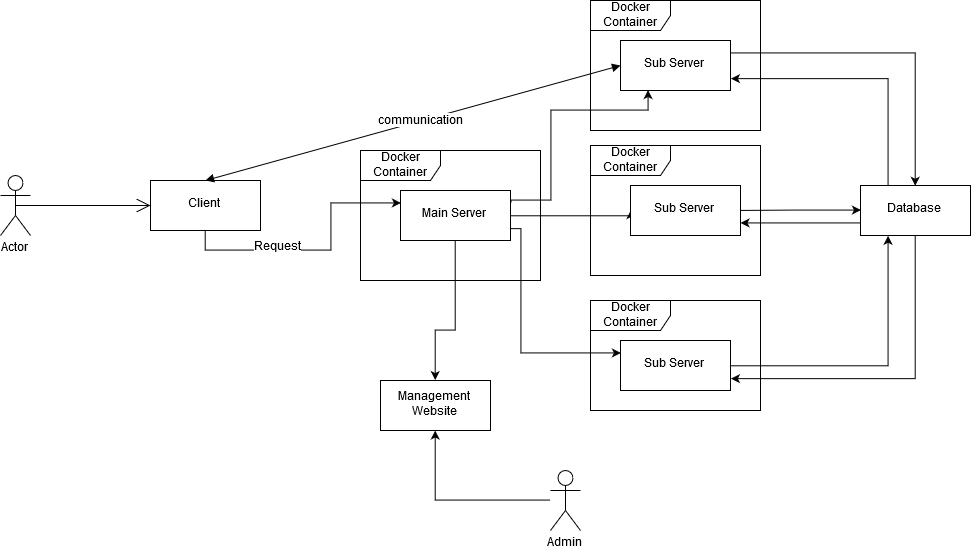
\includegraphics[width=1\linewidth]{Architecture/SysArchitecture.png}
        \caption{System Architecture}
        \label{fig:sysarch}
    \end{figure}
    \begin{text}
    Note: Client can be either a mobile phone or website.
    \end{text}    


\pagebreak
\section{Acceptance Criteria}
    \subsection{Acc 001: Creating and listen to an audio guide}
    \label{sec:acc001}
    \begin{tabular}{|p{.3\linewidth}|p{.7\linewidth}|}
        \hline
        \cellcolor[gray]{0.5}\textcolor{white}{Steps} & \cellcolor[gray]{0.5}\textcolor{white}{Expected behaviour} \\ \hline
        Create a guide & If some input fields are not correctly handled, the guide should not be created. If everything is correct the guide should be created an available \\ \hline
        Listen to that guide & If the user is near the place where the tracks of the guide are located, the guide should appear in the explorer view. If the user clicks on the start guide button, the first track should be played. \\ \hline
        Move to the next track & If the user is near the next track it should be played automatically or the app should make a notification (depending on the settings) \\ \hline
    \end{tabular}
    
    \subsection{Acc 002: Extended Settings of Guide Creation}
    \begin{tabular}{|p{.3\linewidth}|p{.7\linewidth}|}
        \hline
        \cellcolor[gray]{0.5}\textcolor{white}{Steps} & \cellcolor[gray]{0.5}\textcolor{white}{Expected behaviour} \\ \hline
        Create guide & Guide should be created if the user typed in everything correctly. Furthermore, the verified user-defined a price for that guide \\ \hline
        Start listening & Before begin listening the user have to pay the amount that the creator has defined. \\ \hline
        Create a further guide & If an official user disabled the creation of guide near his area near that place the guide should not be created \\ \hline
    \end{tabular}

    \subsection{Acc 003: Rate a guide}
    \begin{tabular}{|p{.3\linewidth}|p{.7\linewidth}|}
        \hline
        \cellcolor[gray]{0.5}\textcolor{white}{Steps} & \cellcolor[gray]{0.5}\textcolor{white}{Expected behaviour} \\ \hline
        Listen to a guide & the user should be able to listen to the tracks. \\ \hline
        Rating & After the user finished or cancelled the guide, he should be able to give that guide starts (from 1 to 5) \\ \hline
        Look at the guide description & After rating, the guide's rating should be updated in the guide view \\ \hline
    \end{tabular}
    
    \subsection{Acc 004: Report a guide}
    \begin{tabular}{|p{.3\linewidth}|p{.7\linewidth}|}
        \hline
        \cellcolor[gray]{0.5}\textcolor{white}{Steps} & \cellcolor[gray]{0.5}\textcolor{white}{Expected behaviour} \\ \hline
        Listen to a guide & the user should be able to listen to the tracks. \\ \hline
        Report & After listening (or cancelling) the user should be able to report the guide. After reporting that guide should be appear on the reported guide list on the admins account. \\ \hline
        Review reported guide & The admin should now be able to review that guide \\ \hline
    \end{tabular}
    
    \subsection{Acc 005: Guide Management}
    \begin{tabular}{|p{.3\linewidth}|p{.7\linewidth}|}
        \hline
        \cellcolor[gray]{0.5}\textcolor{white}{Steps} & \cellcolor[gray]{0.5}\textcolor{white}{Expected behaviour} \\ \hline
        Listen to a guide & the user should be able to listen to the tracks. \\ \hline
        Report & After listening (or cancelling) the user should be able to report the guide. After reporting that guide should appear in the reported guide list on the admins account. \\ \hline
    \end{tabular}
    
    \subsection{Acc 006: Admin User Management}
    \begin{tabular}{|p{.3\linewidth}|p{.7\linewidth}|}
        \hline
        \cellcolor[gray]{0.5}\textcolor{white}{Steps} & \cellcolor[gray]{0.5}\textcolor{white}{Expected behaviour} \\ \hline
        Review Reported Guides & An admin should be able to review a guide that was reported by a user. \\ \hline
        Disable/Delete Guide & According to the outcome of the guide review by the admin he has to act accordingly and, if the report is justified, disable/delete the guide. \\ \hline
        Ban Users & If a User has been reported several times on a bunch of guides, and the review has proven to be justified by an admin, an admin can choose to ban the user.\\ \hline
    \end{tabular}

\end{document}  